Benchmarking-delens fremmeste formål er at finde svar på en række spørgsmål
inden udregningen sættes igang.  Reelt har vi kun en enkelt parameter vi kan
skrue på, nemlig $m$ - antallet af dronninger vi placerer på hver board før vi
genererer et mig job til at regne videre på det board.  Hvilket forhold mellem 
\fixme{what?}
%\subsection{Takaken}
%\subsection{Java port}
%\subsection{Java port v2}
%\subsubsection{Rekursion vs. Iterativ metode}
%\subsubsection{Iterativ med checkpoints}
%\subsection{MiGrid}

\subsection{Lokale tests}

Vi starter med at teste de forskellige udgaver af koden lokalt, så vi har en
baseline at sammenligne med.

Alle lokale tests er kørt på en IBM T43, med en pentium m 1.86Ghz cpu, 

Java koden er kompilet med javac

\begin{verbatim}
alex@roadrunner:~/temp/queens/src/main/java$ javac -version
javac 1.5.0_11
\end{verbatim}

C koden er kompilet med \texttt{gcc -Os -O2 -o nq nqueens.c}

\begin{verbatim}
alex@roadrunner:~/temp/queens/src/main/java$ gcc --version
gcc (GCC) 4.1.2 (Ubuntu 4.1.2-0ubuntu4)
\end{verbatim}

De første tests er kørt på revision 77 (i forbindelse med den iterative test er
udskrivning af debug info til skærmen dog blevet kommenteret ud)

\begin{figure}[h]
\begin{center}
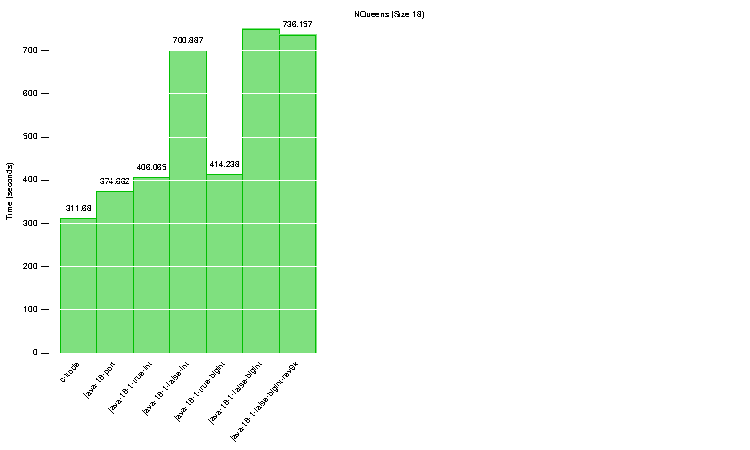
\includegraphics{../benchmarks/lokal.pdf}
\caption{Sammenligning af de lokale test} 
\label{figur:lokal}
\end{center}
\end{figure}

Som det ses er C udgaven en smule hurtigere end den direkte java port, der igen
er lidt hurtigere end den paralleliserede udgave af koden, når den kører
rekursivt. Den iterative udgave er væsentlig langsommere..

Den parallelle udgave af koden er i dette tilfælde her kørt med
\texttt{maxSteps} på 1. 
\begin{figure}[h]
\begin{center}
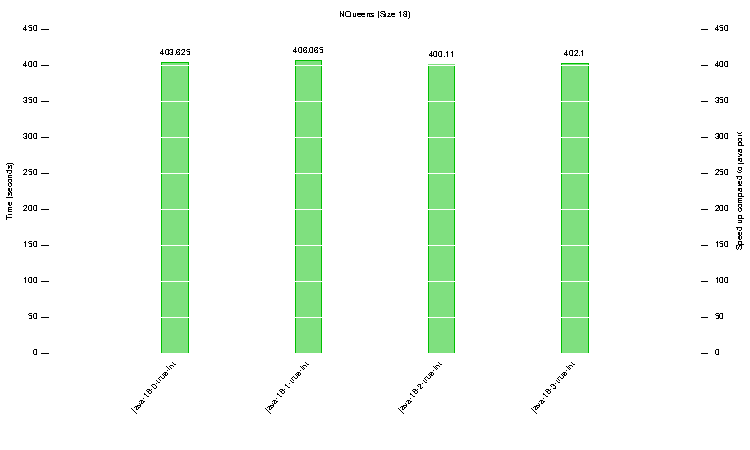
\includegraphics{../benchmarks/maxsteps.pdf}
\caption{insert proper caption here } 
\label{figur:maxsteps}
\end{center}
\end{figure}

På figur \ref{figur:maxsteps} er vidst kørsler for $n=18$ for forskellige
$maxSteps$. 
Som det ses, har det ikke den store indflydelse på performance hvor stor
$maxSteps$ er, der er altså ikke det store overhead ved at generere en masse
opgaver og løse dem bagefter, når det kører lokalt. 

Det skal også nævnes at for $maxSteps>n/2$ vil vores program regne forkert.
Dette skyldes \fixme{ja.. hvad skyldes det.. }


I tabel \ref{tabel:noboards} kan det ses hvor mange boards der bliver genereret
for forskellige $n$ og $maxSteps$. 

\fixme{hvor mange jobs bliver der lavet for de forskellige maxsteps, indsæt
tabel?}
\begin{table}
	\begin{center}
		\begin{tabular}{|c|c|c|c|c|c|}
			\hline N  & maxSteps  & boards & n  & maxSteps & boards \\
			\hline 15 & 0         & 18     & 17 & 0        & 21     \\
			\hline 15 & 1         & 173    & 17 & 1        & 243    \\
			\hline 15 & 2         & 1310   & 17 & 2        & 2282   \\ 
			\hline 15 & 3         & 8349   & 17 & 3        & 18161  \\
			\hline 15 & 4         & 43961  & 18 & 0        & 23     \\
			\hline 16 & 0         & 20     & 18 & 1        & 289    \\
			\hline 16 & 1         & 212    & 18 & 2        & 2983   \\
			\hline 16 & 2         & 1797   & 18 & 3        & 26204  \\
			\hline 16 & 3         & 12840  &    &          &        \\
			\hline 16 & 4         & 76224  &    &          &        \\
			\hline
		\end{tabular}
		\caption{Antal Boards der bliver genereret}
		\label{tabel:noboards}
	\end{center}
\end{table}

\begin{table}
	\begin{center}
		\begin{tabular}{|c|c|c|}
			\hline N & unikke & totale \\
			\hline 15 & 285053 & 2279184 \\
			\hline 16 & 1846955 & 14772512 \\
			\hline 17 & 11977939 & 95815104  \\
			\hline 18 & 83263591 & 666090624 \\
			\hline
		\end{tabular}
		\caption{Antal Boards der bliver genereret}
		\label{tabel:unikkevstotale}
	\end{center}
\end{table}

\begin{figure}[h]
\begin{center}
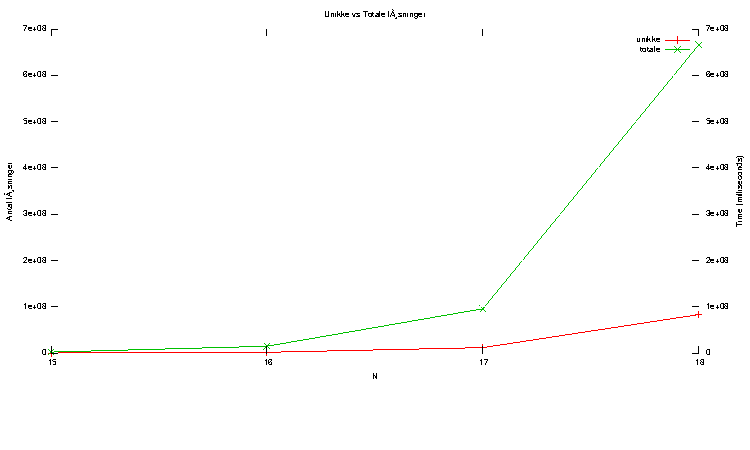
\includegraphics{../benchmarks/unikkevstotale.pdf}
\caption{Unikke og totale antal løßninger} 
\label{figur:unikkevstotale}
\end{center}
\end{figure}

Alle tests er i første omgang kørt 5 gange, dette blev gjort for at se om
køretiden svingede meget, da dette ikke lader til at være tilfældet (se figur
\ref{figur:b1} vil resten af testene kun blive kørt 1 gang.. 

\begin{figure}[h]
\begin{center}
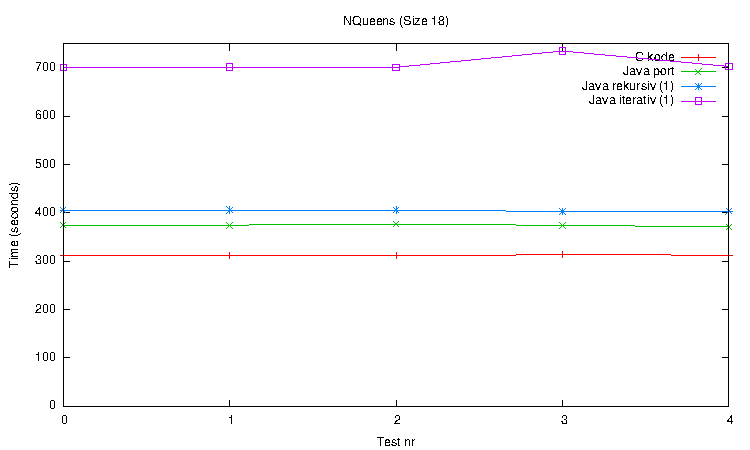
\includegraphics{../benchmarks/b1.pdf}
\caption{insert proper caption here } 
\label{figur:b1}
\end{center}
\end{figure}

Nu skal vi så se på hvor hurtigt det kører når vi smider det efter MiGrid. 
Disse tests er kørt med \texttt{maxSteps} 0 og 1.

\fixme{indsaet en graf, eller bare resultaterne og henvis til b3?}
De foregående tests er kørt med kode der bruger \texttt{int} til at gemme resultaterne,
i de næste tests er \texttt{int} skiftet ud med \texttt{BigInteger} 
Her er den rekursive test kørt på revision 83, og den iterative er kørt på
revision 9x. At den iterative er kørt på en anden revision skyldes at der i den
iterative kode var en debug linje der ikke var blevet kommenteret ud, der gjorde
at koden kørte utroligt langsomt.

Som det kan ses på figur \ref{figur:lokal} kører den rekursive kode en smule
langsommere med \texttt{BigInteger} end med \texttt{int}, hvor tiden stiger fra
406.065 til 414.238, hvilket svarer til en forøgelse
på knap 2\% \fixme{hva' med den iterative}


\subsection{kald til backtrack}

Hvis man ser på antallet af kald til backtrack de forskellige versioner laver,
er de ens for c koden og den direkte java port, og hvis man kører med
$maxSteps=0$ er antallet af kald for den parallele og iterative kode også det
samme som for c koden (se tabel \ref{tabel:backtrackkald}. Med $maxSteps>0$ får
vi færre kald til backtrack, hvilket skyldes at en del af disse kald bliver
lavet i forbindelse med oprettelsen af de ekstra boards. 

\begin{table}
\begin{center}
\begin{tabular}{|c|c|c|}
\hline kodebase  & hjørnebrædt & midtebrædt \\
\hline C kode    &  748267           &  5293206           \\
\hline Java      &  748267           &  5293206           \\
\hline Java rek. &  748267           &  5293206           \\
\hline Java ite. &  748267           &  5293206           \\
\hline
\end{tabular}
\caption{Kald til backtrack for $n=14$}
\label{table:backtrackkald}
\end{center}
\end{table}

\subsection{Jobstørrelse}

Med jobstørrelse refererer vi til hvor lang tid det tager at løse et job, og
ikke størrelsen på data. 
Som det ses i \ref{tabel:jobsize}, varierer jobstørrelsen
meget. Cornerboards er generelt ret små, mens middleboards er generelt er en del
større. Det ses også i tabellen at jobstørrelsen afhænger af de bounds der er i
henholdsvist MiddleBoard og CornerBoard. Hvis man øger $maxSteps$ og dermed får
lavet flere jobs, ses det at de enkelte jobs bliver delt op i nogenlunde lige
støre dele, den relative størrelse mellem det mindste og største jobs er dog
stadig nogenlunde det samme. \fixme{lav en benchmark/beregning der viser dette?}

\subsection{Generering af jobs}

Generering og indsendelse af jobs afhænger tildels af den internetforbindelse
man sidder på, da indsendelse jo går via internettet. De forskellige jobs vi har
submitted til MiGrid har genereringen og indsendelse af jobs svinget fra xx til
xx (se tabel \ref{tabel:jobgenerering}) \fixme{lav den fscking tabel og skriv de
rigtige tal ind}. Langt den største del af tiden går også med at sende jobsne,
da genereringen af jobs for større mængder jobs tager ca 0.01ms/job
\begin{table}
\begin{center}
\begin{tabular}{|c|c|c|c|c|}
\hline N & maxSteps & tid (ms) & brædt & tid (ms) /brædt \\
\hline 17 & 0 & 4 & 21 & 0.19 \\
\hline 17 & 1 & 6 & 243 & 0.02 \\
\hline 17 & 2 & 23 & 2282 & 0.01 \\
\hline 17 & 3 & 206 & 18161 & 0.01 \\
\hline 17 & 4 & 1252 & 121116 & 0.01 \\
\hline 18 & 0 & 4 & 23 & 0.17 \\
\hline 18 & 1 & 6 & 239 & 0.02 \\
\hline 18 & 2 & 44 & 2983 & 0.01 \\
\hline 18 & 3 & 280 & 26204 & 0.01 \\
\hline
\end{tabular}
\caption{Tid for generering af brædt}
\label{table:boardgenering}
\end{center}
\end{table}
\fixme{lav det om til en tabel.. der}

\subsection{Kørsel på \mig}

Den reelle køretid på \mig findes ved at tage \texttt{Queued} tiden for det første job der er
blevet sat i kø, og \texttt{Finished} tiden for det sidste job der er blevet
færdigt, og så finde forskellen.

\subsubsection{Overhead ved jobskifte}

I MiG\_main() metoden i NQueenJob laver vi et timestamp i starten og slutningen
af metoden.  og kan så tage start tiden for et job og trække sluttiden for det
foregående job fra, og man har så et estimat for hvor lang tid et jobskifte
tager, vi har gjort dette for 8 jobs, og får så 7 estimater, gennemsnittet af
dem bliver 18.455 sek.  Op til 15 af disse 18 sekunder, skyldes at oneclick
applet'en sover i 15 sekunder.  Ved en kørsel med $n=18$ og $maxSteps=1$, hvor
vi så får 289 jobs, giver det knap 89 minutter. En del af dette overhead vil
selvfølgelig blive "gemt", når der er flere ressourcer der kører samtidigt.

